%
% To start the document, use
%  \chapter{...}
% For lover level, sections use
%  \section{...}
%  \subsection{...}
%
\chapter{Gridded Fields}
%-------------------------------------------------------------------------
\label{sec:griddedfields}


%
% Document history, format:
%  \starthistory
%    date1 & text .... \\
%    date2 & text .... \\
%    ....
%  \stophistory
%
\starthistory
  2010-09-28 & Oliver Lemke: Updated for implementation changes.\\
  2010-04-12 & Created and written by Oliver Lemke.\\
\stophistory




%
% Introduction
%

This section describes how gridded fields are implemented in ARTS and
how they are used. Gridded fields consist of a data object like a
Vector, Matrix, or Tensor and a grid for each dimension of its data.
For example, a \builtindoc{GriddedField1} consists of one grid and a
\builtindoc{Vector}, whereas a \builtindoc{GriddedField3} contains three grids
and a \builtindoc{Tensor3}. Grids can be either numeric, like a pressure grid,
or strings, like channel names.


\section{Implementation files}
%-------------------------------------------------------------------------
\label{sec:griddedfields:files}

The \builtindoc{GriddedField1}, \builtindoc{GriddedField2},
\builtindoc{GriddedField3}, \builtindoc{GriddedField4} classes and their common
base class \shortcode{GriddedField} described below reside in the files:

\begin{itemize}
\item \fileindex{gridded\_fields.h}
\item \fileindex{gridded\_fields.cc}
\end{itemize}

\section{Design}
%-------------------------------------------------------------------------
\label{sec:griddedfields:design}



\subsection{The abstract base class \shortcode{GriddedField}}
%-------------------------------------------------------------------------

The abstract base class \shortcode{GriddedField} implements the properties
all gridded fields have in common. These are mostly the methods to create,
set, and access the grids. A \shortcode{GriddedField} is never instantiated
directly.


\subsection{Inheritance}
%-------------------------------------------------------------------------

The \shortcode{GriddedFieldX} classes use indirect inheritance to combine a
data object with the grids, see Figure \ref{fig:griddedfields:uml}.

\begin{figure}[ht!]
\begin{center}
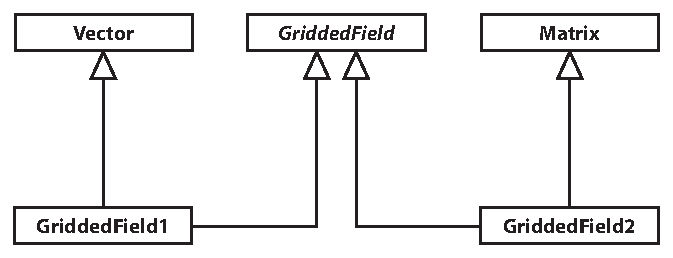
\includegraphics{Figs/development/griddedfields_inheritance}
\caption{UML diagram of gridded field inheritance.}
\label{fig:griddedfields:uml}
\end{center}
\end{figure}


\section{Constructing Gridded Fields}
%-------------------------------------------------------------------------
\label{sec:griddedfields:construct}


\subsection{Creation}
%-------------------------------------------------------------------------
\label{sec:griddedfields:create}

Each \shortcode{GriddedFieldX} offers two constructors. One default
constructor that creates an unnamed gridded field and a second constructor
that takes a string with the name of the gridded field as an argument.

\begin{code}
GriddedField1 gfone("I'm a GriddedField1");
GriddedField2 gftwo;

gftwo.set_name ("I'm a GriddedField2");
\end{code}


\subsection{Initializing the grids}
%-------------------------------------------------------------------------
\label{sec:griddedfields:initgrids}

Once a gridded field has been created, we can start setting up the
grids. There are two different types of grids, a numeric grid and a
string grid. In the following example we set up two gridded fields: A
\builtindoc{GriddedField1} with a numeric grid and a \builtindoc{GriddedField2}
with a numeric grid for the rows and a string grid for the columns. Each grid
can be assigned a name to describe its contents or unit.

\begin{code}
Vector gfonegrid(1,5,1);        // gfonegrid = [1,2,3,4,5]
gfone.set_grid(0, gfonegrid);   // Set grid for the vector elements.

Vector gftwogrid0(1,5,1);       // gftwogrid0 = [1,2,3,4,5]
ArrayOfString gftwogrid1{"Chan1", "Chan2", "Chan3"};

gftwo.set_grid(0, gftwogrid0);  // Set grid for the matrix rows.
gftwo.set_grid(1, gftwogrid1);  // Set grid for the matrix columns.

gfone.set_grid_name (0, "Pressure");

gftwo.set_grid_name (0, "Pressure");
gftwo.set_grid_name (1, "Channel");
\end{code}

\subsection{Initializing the data}
%-------------------------------------------------------------------------
\label{sec:griddedfields:initdata}

The data of a \shortcode{GriddedFieldX} can be accessed through its \shortcode{data} member.
For a \builtindoc{GriddedField1} \shortcode{data} is a \builtindoc{Vector}, for a \builtindoc{GriddedField2} a \builtindoc{Matrix}, for a \builtindoc{GriddedField3} a \builtindoc{Tensor3}, and so on.

The following code shows how to fill the gridded fields from the previous example with data:

\begin{code}
Vector avector(1,4,0.5);    // avector = [1,1.5,2,2.5]

gfone.data = avector;

Matrix amatrix(5,3,4.);     // amatrix = [[4,4,4],[4,4,4],...]

gftwo.data = amatrix;
\end{code}

\subsection{Consistency check}
%-------------------------------------------------------------------------
\label{sec:griddedfields:consistency}

After initializing or changing either the grids or the data, it can happen
that the size of the grids does not match the size of the data anymore. Each
gridded field provides a convenience function which can be called to perform a
consistency check.

\begin{code}
if (!gfone.checksize())
  cout << gfone.get_name()
       << ": Sizes of grid and data don't match" << endl;

// This should fail!
if (!gftwo.checksize())
  cout << gftwo.get_name()
       << ": Sizes of grids and data don't match" << endl;
\end{code}

The complete source code of the examples from this chapter can be found in
\shortcode{src/test\_gridded\_fields.cc}.

%%% Local Variables:
%%% mode: latex
%%% TeX-master: "arts_developer"
%%% End:

